\documentclass[fleqn]{article}
\usepackage[english]{babel}
\usepackage{amsmath}
\usepackage{amsthm}
\usepackage{graphicx}
\usepackage[utf8]{inputenc}

%%%%%%%% MARGIN
\usepackage[left=1in, right=1in, top=0.8in, bottom=0.8in]{geometry}

%%%%%%%% NO PARAGRAPH INDENT
% https://tex.stackexchange.com/questions/27802/set-noindent-for-entire-file
\setlength\parindent{0pt}

%%%%%%%% SUB-FIGURE PACKAGE
\usepackage{subcaption}

\usepackage{pdfpages}

%%%%%%%% HYPERREF PACKAGE
\usepackage{hyperref}
\hypersetup{linkcolor=blue}
\hypersetup{citecolor=blue}
\hypersetup{urlcolor=blue}
\hypersetup{colorlinks=true}

%%%%%%%% MULTI-COLUMNS PACKAGE
\usepackage{multicol}

%%%%%%%% SETS DEFINITIONS
\usepackage{amssymb}
%%%% Important sets
\renewcommand{\O}{\mathbb{O}}
\newcommand{\N}{\mathbb{N}}
\newcommand{\Z}{{\mathbb{Z}}}
\newcommand{\Q}{{\mathbb{Q}}}
\newcommand{\RR}{{\mathbb{R}}}

%%%% Statistics
\newcommand{\E}[1]{\mathbb{E}\left[#1 \right]}
\newcommand{\V}[1]{\mathbb{V}\left[#1 \right]}
\newcommand{\cov}[1]{\mathrm{Cov}\left[#1 \right]}

%%% Misc Math
% Spaces after/before left/right
\let\originalleft\left
\let\originalright\right
\renewcommand{\left}{\mathopen{}\mathclose\bgroup\originalleft}
\renewcommand{\right}{\aftergroup\egroup\originalright}

% Norm and abs
\newcommand{\norm}[1]{\left\lVert#1\right\rVert}
\newcommand{\abs}[1]{\left\lvert#1\right\rvert}

%%%% Superscript to the left
% https://latex.org/forum/viewtopic.php?t=455
\usepackage{tensor}
\newcommand{\app}[3]{\tensor*[^{#1}]{\left(#2, #3\right)}{}}


%%%%%%%% SPLIT EQUATIONS
% https://tex.stackexchange.com/questions/51682/is-it-possible-to-pagebreak-aligned-equations
\allowdisplaybreaks

%%%%%%%% CODE RENDERING
% Compile with flag -shell-escape
\usepackage{minted}

%%%%%%%% EXAM PACKAGE
\usepackage{mathexam}

%%%%%%%% CHANGE MARGINS ITEMIZE
\usepackage{enumitem}

%%%%%%%% START DOCUMENT

\ExamClass{EC0301 - Time Series}
\ExamName{Assignment \#10}
\ExamHead{\today}

\let\ds\displaystyle

\begin{document}
 \vspace{0.3cm}
   % Information of the student
   \begin{itemize}[leftmargin=6.25cm, labelsep=0.5cm]

     \item[\textit{Name}] \scalebox{1.2}{David Plazas Escudero} % Name
     \item[\textit{Student code}] 201710005101 % Code

   \end{itemize}
\vspace{0.3cm}

% Each of the items to solve
\begin{enumerate}
    \item \textit{Show that the difference of a series with a step variable is a series with an impulse variable.}
    
    Let us consider the series in the form 
    \[
    \phi(L)x_t=\theta(L)\epsilon_t + \omega_0E_t,
    \]
    where
    \[
    E_t=\begin{cases}
    0, & t < t^*\\
    1, & t \geq t^*
    \end{cases}
    \]
    is the unitary step at $t^*$. This series can be equivalently rewritten as 
    \[
    x_t=\sum_{r=1}^p\phi_rx_{t-r}+\epsilon_t-\sum_{r=1}^q\theta_r\epsilon_{t-r}+\omega_0E_t.
    \]
    Let $w_t:=\Delta x_t=x_t-x_{t-1}$, then
    \[
    \begin{split}
    w_t&=\sum_{r=1}^p\phi_rx_{t-r}+\epsilon_t-\sum_{r=1}^q\theta_r\epsilon_{t-r}+\omega_0E_t - \sum_{r=1}^p\phi_rx_{t-r-1}-\epsilon_{t-1}+\sum_{r=1}^q\theta_r\epsilon_{t-r-1}-\omega_0E_{t-1}\\
    &=\sum_{r=1}^p\phi_r(x_{t-r}-x_{t-r-1})+\epsilon_t-\left[\sum_{r=1}^q\theta_r\epsilon_{t-r}+\epsilon_t-\sum_{r=1}^q\theta_r\epsilon_{t-r-1}\right]+\omega_0(E_t-E_{t-1}).
    \end{split}
    \]
    The expression inside the square brackets can be re-arranged into a new MA($q$) model with different coefficients. Thus,
    \[
    w_t=\sum_{r=1}^p\phi_rw_{t-r}+\epsilon_t-\sum_{r=1}^q\tilde{\theta}_r\epsilon_{t-r}+\omega_0(E_t-E_{t-1}),
    \]
    and this series can be written as
    \[
    \phi(L)w_t=\tilde{\theta}(L)\epsilon_t+\omega_0(E_t-E_{t-1}).
    \]
    Now, let us prove that $E_t-E_{t-1}$ is an equivalent definition of the unitary impulse. The function $E_{t-1}$ is 
    \[
    E_{t-1} = \begin{cases}
    0, & t-1 < t^*\\
    1, & t-1 \geq t^*
    \end{cases}=\begin{cases}
    0, & t < t^*+1\\
    1, & t \geq t^*+1
    \end{cases},
    \]
    then, the difference $E_t-E_{t-1}$ can be seen as a piecewise function defined on three intervals: 
    \[
    E_t-E_{t-1} = \begin{cases}
    0-0, & t < t^*\\
    1-0, & t^* \leq t < t^*+1\\
    1-1, & t\geq t^*+1
    \end{cases}
    \]
    Considering that we are working in discrete-time, this function can be rewritten as
    \[
    E_t-E_{t-1} = \begin{cases}
    0, & t \neq t^*\\
    1, & t = t^*
    \end{cases}=I_t
    \]
    which is exactly the definition of the unitary impulse function. Then, the first difference of series with a step variable is
    \[
    \phi(L)w_t=\tilde{\theta}(L)\epsilon_t+\omega_0I_t.
    \]
    
    \item \textit{Using the data from ``dataUK.xlsx'', estimate an ADL(1,1) model for the interest rate of the Central Bank of England with the ``economy feeling'' as the exogenous variable. Which model is better to represent the series data?}
    
    The code for this exercise is:
    \begin{minted}{R}
    library(readxl)
    library(dynlm)
    data <- read_excel("dataUK.xlsx")
    
    x <- ts(data$`interest rate`)
    z <- ts(data$`eco sent`)
    
    model <- dynlm(x ~ L(x, 1) + z + L(z, 1))
    \end{minted}
    and the resulting model object is presented in Figure \ref{fig:model}. Note that both $\beta_0$ and $\beta_1$ are close to zero. In the case were $\beta_0=\beta_1=0$, the ADL(1,1) model is equivalent to an AR(1) model. Hence, an AR(1) model can better fit the series data.
    
    \begin{figure}[H]
        \centering
        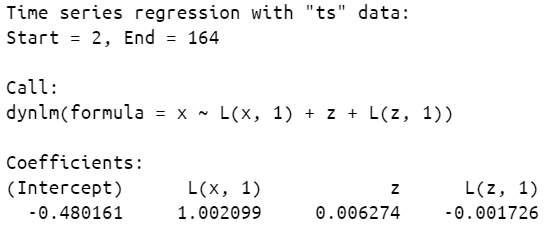
\includegraphics[scale=0.7]{figs/model.png}
        \caption{Model results.}
        \label{fig:model}
    \end{figure}
    \item \textit{Using the interest rate data from ``dataUK.xlsx'', estimate the optimal breakpoints in two scenarios: i) fixing 1 breakpoint, ii) let the algorithm estimate the number of optimal breakpoints (non-fixed number of breakpoints).}
    
    The code for both scenarios is:
    \begin{minted}{R}
    library(strucchange)
    
    # 1 break point
    breakpoints(x ~ 1, breaks=1)
    
    # n break points
    breakpoints(x ~ 1)
    \end{minted}
    The results for fixing 1 break are presented in Figure \ref{fig:1} and for the second scenario in Figure \ref{fig:n}. The series data is presented in Figure \ref{fig:ts}. Clearly, the first scenario (1 breakpoint) better represents the series data, since it presents a clear breakpoint around 59, as estimated; whereas the second scenario clearly is overestimating the breakpoint, considering some minor outliers as breakpoints.
    \begin{figure}[H]
    \centering
    \begin{subfigure}[b]{0.45\textwidth}
        \centering
        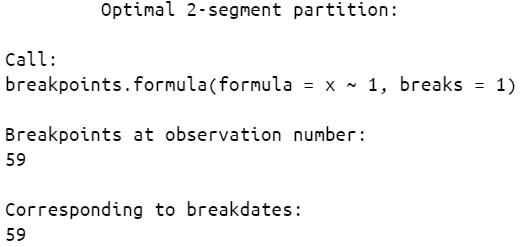
\includegraphics[width=\textwidth]{figs/1.png}
        \caption{1 breakpoint.}
        \label{fig:1}
    \end{subfigure}
    \begin{subfigure}[b]{0.45\textwidth}  
        \centering 
        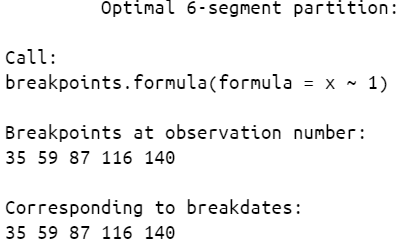
\includegraphics[width=0.8\textwidth]{figs/n.png}
        \caption{Unknown breakpoints.}
        \label{fig:n}
    \end{subfigure}
    \caption{Breakpoint results for the two scenarios.}
    \label{fig:breaks}
\end{figure}
\begin{figure}[H]
        \centering
        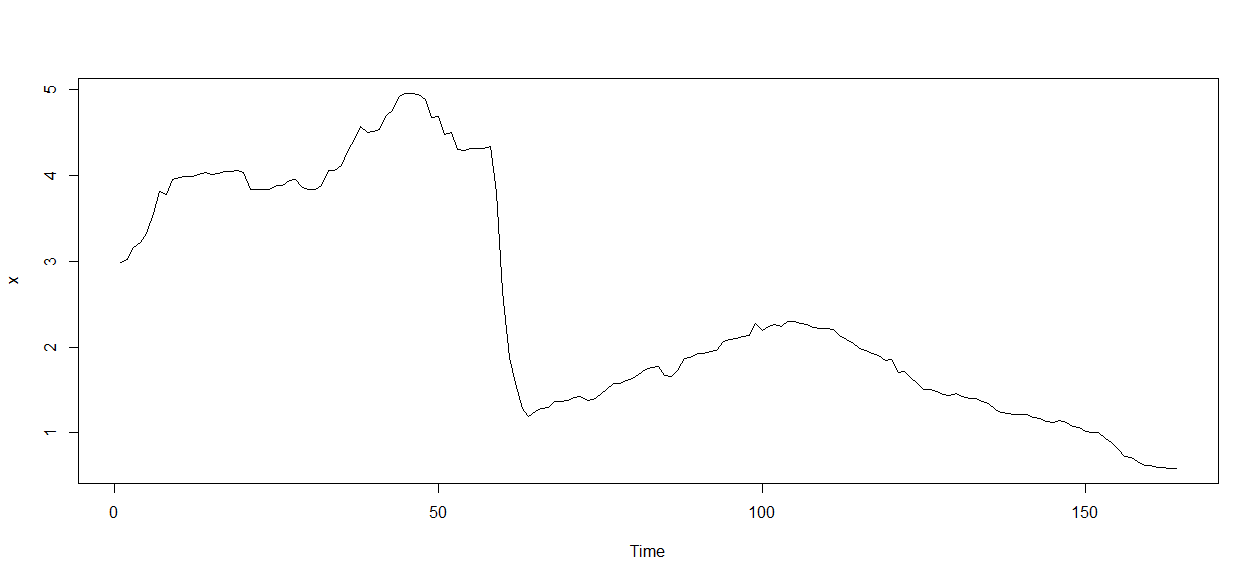
\includegraphics[width=\textwidth]{figs/ts.png}
        \caption{Time series data.}
        \label{fig:ts}
    \end{figure}
\end{enumerate}
\end{document}
